\section{Composite}

Esse padrão fornece uma estrutura de objetos 
organizados como uma árvore, representados 
por uma hierarquia parte-todo. 
Com isso, é possível tratar tanto o conjunto 
quanto os objetos individuais de forma 
uniforme, sem que seja necessário conhecer 
os elementos pertencentes a um conjunto para 
tratá-lo.

A figura \ref{composite_struct} demonstra a 
estrutura do padrão, onde uma interface Component 
define tanto um objeto nó, representado pela 
classe Composite, quanto um objeto folha, 
representado pela classe Leaf. Os elementos 
filhos da classe Composite são todos instâncias 
de Component, o que faz com que a classe não 
saiba se seus filhos são outros objetos compostos 
ou se são objetos folha.

\begin{figure}[htb]
	\caption{\label{composite_struct}Estrutura do Composite}
	\begin{center}
	    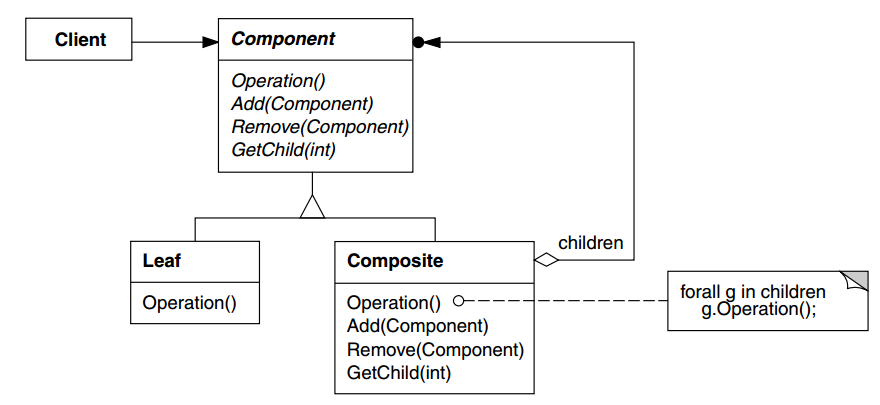
\includegraphics[scale=0.5]{5_padroes-contexto-funcional/5.2_estruturais/5.2.3_composite/diagram.png}
	\end{center}
\end{figure}

\subsection*{Exemplo Orientado a Objetos}

Como exemplo, é apresentada uma ferramenta gráfica 
onde o usuário pode agrupar diversas formas e 
elementos 
para formar diagramas maiores e mais complexos. 
Apesar do usuário tratar esses diagramas como um 
único elemento gráfico, a aplicação precisa levar 
em consideração todos os elementos dos quais ele 
é composto. Dessa forma, o padrão Composite permite 
abstrair os elementos menores, tratando o elemento 
composto como algo único, da mesma forma que 
são tratados os elementos não compostos. A figura 
\ref{composite_exemplo} demonstra o diagrama de 
classes para esse exemplo, enquanto o código 
\ref{oocomposite} traz um exemplo de implementação.

\begin{figure}[htb]
	\caption{\label{composite_exemplo}Exemplo de Composite}
	\begin{center}
	    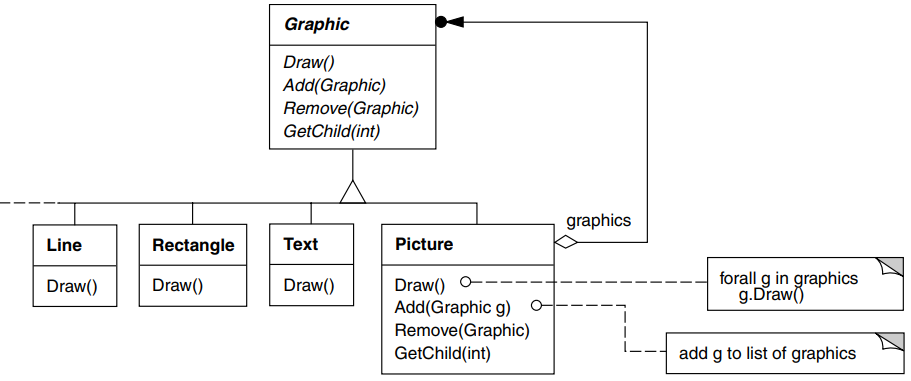
\includegraphics[scale=0.45]{5_padroes-contexto-funcional/5.2_estruturais/5.2.3_composite/exemplo_composite.png}
	\end{center}
\end{figure}

\begin{lstlisting}[caption={Composite Orientado a Objetos},label=oocomposite]

	trait Graphic {
		def Draw();
		def Add(graphic : Graphic);
		def Remove(graphic : Graphic);
		def GetChild(pos : Int) : Graphic;
	}

	class Picture() extends Graphic {
		
		var graphics : List[Graphic]
	
		def Draw() {
			// desenha o elemento na tela
		}

		def Add(graphic : Graphic) {
			graphics.add(graphic);
		}

		def Remove(graphic : Graphic) {
			graphics.remove(graphic);
		}

		def GetChild(pos : Int) {
			return graphics.get(pos);
		}
	}

	class Text() extends Graphic {
		def Draw() {
			// desenha o elemento na tela
		}
	}

	class Rectangle() extends Graphic {
		def Draw() {
			// desenha o elemento na tela
		}
	}

	class Line() extends Graphic {
		def Draw() {
			// desenha o elemento na tela
		}
	}


\end{lstlisting}

\subsection*{Contexto Funcional}



\begin{lstlisting}[caption={Composite Funcional},label=fpcomposite]
    

    
\end{lstlisting}